\documentclass[tikz,border=7pt]{standalone}

\usepackage[T1]{fontenc}
\usepackage[scaled=0.94]{helvet}
\renewcommand{\familydefault}{\sfdefault}
\usetikzlibrary{arrows.meta}

\definecolor{linkgray}{HTML}{374151}
\definecolor{failred}{HTML}{C0392B}
\definecolor{overlayblue}{HTML}{1677B8}
\definecolor{leadergold}{HTML}{F6C85F}
\definecolor{qcblue}{HTML}{DCEEFF}
\definecolor{panelgray}{HTML}{D1D5DB}
\definecolor{textgray}{HTML}{4B5563}

\tikzset{
  replica/.style={circle, draw=linkgray, fill=white, line width=0.7pt,
    minimum size=6.5mm, inner sep=0pt, font=\bfseries\scriptsize},
  leader/.style={replica, fill=leadergold, double=linkgray, double distance=1pt},
  qc/.style={replica, fill=qcblue, line width=1.1pt},
  live/.style={draw=linkgray, line width=1.05pt},
  failed/.style={draw=failred, line width=1.05pt, densely dashed},
  route/.style={draw=overlayblue, line width=2.15pt, opacity=0.86,
    {Stealth[length=2.2mm]}-{Stealth[length=2.2mm]},
    shorten <=3.5mm, shorten >=3.5mm},
  panel/.style={draw=panelgray, rounded corners=2pt, line width=0.55pt},
  rowtitle/.style={anchor=west, font=\bfseries\small},
  tag/.style={anchor=east, font=\scriptsize, text=textgray},
  heading/.style={font=\bfseries\small, text=linkgray},
  note/.style={font=\scriptsize, text=textgray, align=center}
}

% Fixed Omni-Paxos pentagonal arrangement used in every five-node view.
\newcommand{\pentagoncoords}[1]{%
  \coordinate (#1A) at (-1.10,0.30);
  \coordinate (#1B) at (0,1.10);
  \coordinate (#1C) at (1.10,0.30);
  \coordinate (#1D) at (-0.68,-0.90);
  \coordinate (#1E) at (0.68,-0.90);
}

\newcommand{\alllinks}[1]{%
  \foreach \u/\v in {A/B,A/C,A/D,A/E,B/C,B/D,B/E,C/D,C/E,D/E}
    {\draw[live] (#1\u)--(#1\v);}%
}

\newcommand{\fivenodes}[3]{%
  \node[#2]      at (#1A) {A};
  \node[replica] at (#1B) {B};
  \node[#3]      at (#1C) {C};
  \node[replica] at (#1D) {D};
  \node[replica] at (#1E) {E};
}

\newcommand{\betweenarrow}{%
  \draw[-{Stealth[length=2.4mm]},draw=panelgray,line width=1.4pt]
    (-0.35,0.15)--(0.35,0.15);
}

\begin{document}
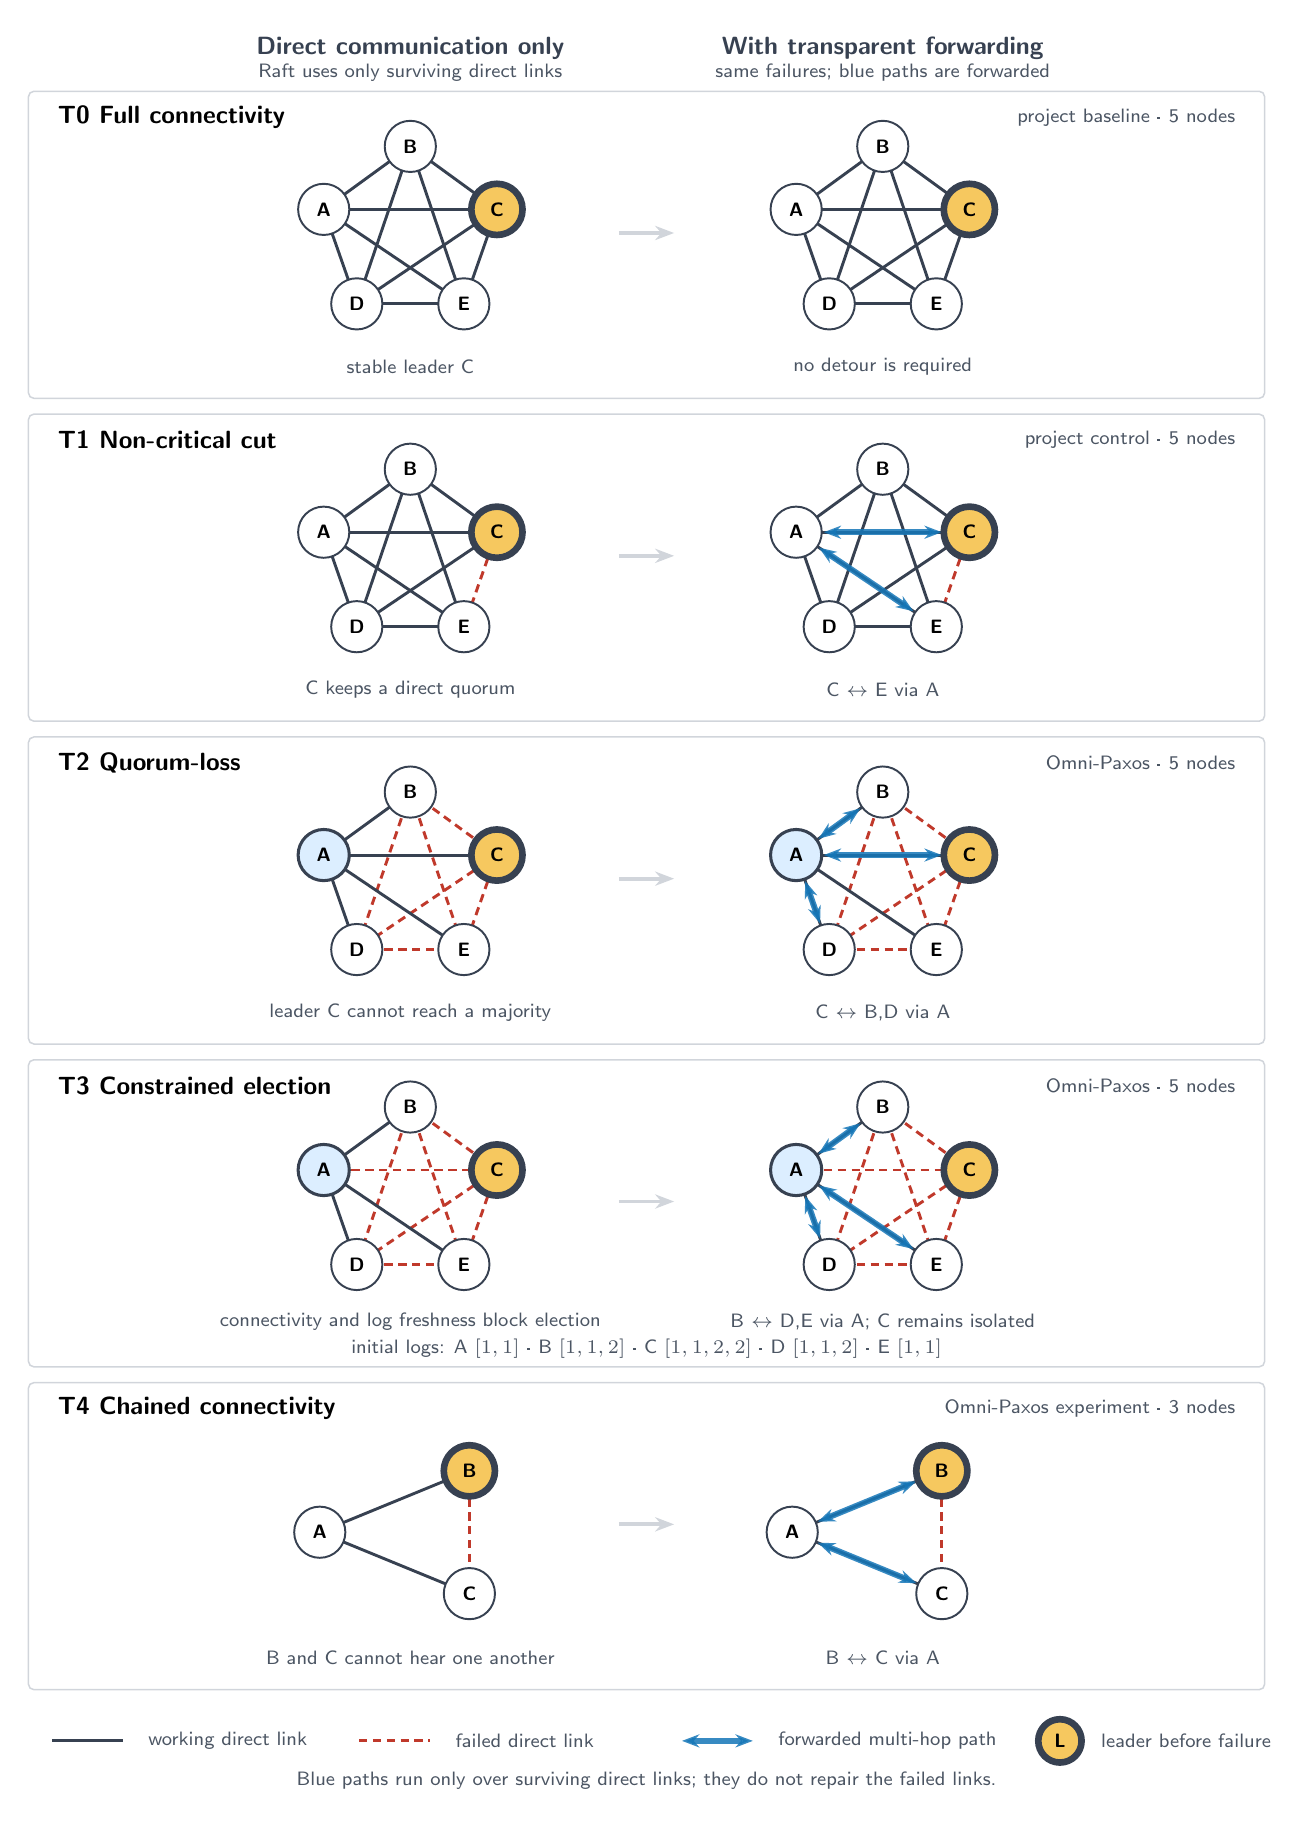
\begin{tikzpicture}[x=1cm,y=1cm]

\node[heading] at (-3,11.15) {Direct communication only};
\node[note] at (-3,10.84) {Raft uses only surviving direct links};
\node[heading] at (3,11.15) {With transparent forwarding};
\node[note] at (3,10.84) {same failures; blue paths are forwarded};

% T0 -------------------------------------------------------------------------
\begin{scope}[shift={(0,8.65)}]
  \draw[panel] (-7.85,-1.95) rectangle (7.85,1.95);
  \node[rowtitle] at (-7.60,1.62) {T0  Full connectivity};
  \node[tag] at (7.60,1.62) {project baseline · 5 nodes};

  \begin{scope}[shift={(-3,0.15)}]
    \pentagoncoords{t0d}
    \alllinks{t0d}
    \fivenodes{t0d}{replica}{leader}
  \end{scope}
  \betweenarrow
  \begin{scope}[shift={(3,0.15)}]
    \pentagoncoords{t0o}
    \alllinks{t0o}
    \fivenodes{t0o}{replica}{leader}
  \end{scope}
  \node[note] at (-3,-1.55) {stable leader C};
  \node[note] at (3,-1.55) {no detour is required};
\end{scope}

% T1 -------------------------------------------------------------------------
\begin{scope}[shift={(0,4.55)}]
  \draw[panel] (-7.85,-1.95) rectangle (7.85,1.95);
  \node[rowtitle] at (-7.60,1.62) {T1  Non-critical cut};
  \node[tag] at (7.60,1.62) {project control · 5 nodes};

  \begin{scope}[shift={(-3,0.15)}]
    \pentagoncoords{t1d}
    \foreach \u/\v in {A/B,A/C,A/D,A/E,B/C,B/D,B/E,C/D,D/E}
      {\draw[live] (t1d\u)--(t1d\v);}
    \draw[failed] (t1dC)--(t1dE);
    \fivenodes{t1d}{replica}{leader}
  \end{scope}
  \betweenarrow
  \begin{scope}[shift={(3,0.15)}]
    \pentagoncoords{t1o}
    \foreach \u/\v in {A/B,A/C,A/D,A/E,B/C,B/D,B/E,C/D,D/E}
      {\draw[live] (t1o\u)--(t1o\v);}
    \draw[failed] (t1oC)--(t1oE);
    \draw[route] (t1oC)--(t1oA);
    \draw[route] (t1oA)--(t1oE);
    \fivenodes{t1o}{replica}{leader}
  \end{scope}
  \node[note] at (-3,-1.55) {C keeps a direct quorum};
  \node[note] at (3,-1.55) {C $\leftrightarrow$ E via A};
\end{scope}

% T2 -------------------------------------------------------------------------
\begin{scope}[shift={(0,0.45)}]
  \draw[panel] (-7.85,-1.95) rectangle (7.85,1.95);
  \node[rowtitle] at (-7.60,1.62) {T2  Quorum-loss};
  \node[tag] at (7.60,1.62) {Omni-Paxos · 5 nodes};

  \begin{scope}[shift={(-3,0.15)}]
    \pentagoncoords{t2d}
    \foreach \u/\v in {B/C,B/D,B/E,C/D,C/E,D/E}
      {\draw[failed] (t2d\u)--(t2d\v);}
    \foreach \u/\v in {A/B,A/C,A/D,A/E}{\draw[live] (t2d\u)--(t2d\v);}
    \fivenodes{t2d}{qc}{leader}
  \end{scope}
  \betweenarrow
  \begin{scope}[shift={(3,0.15)}]
    \pentagoncoords{t2o}
    \foreach \u/\v in {B/C,B/D,B/E,C/D,C/E,D/E}
      {\draw[failed] (t2o\u)--(t2o\v);}
    \foreach \u/\v in {A/B,A/C,A/D,A/E}{\draw[live] (t2o\u)--(t2o\v);}
    \foreach \u/\v in {C/A,A/B,A/D}{\draw[route] (t2o\u)--(t2o\v);}
    \fivenodes{t2o}{qc}{leader}
  \end{scope}
  \node[note] at (-3,-1.55) {leader C cannot reach a majority};
  \node[note] at (3,-1.55) {C $\leftrightarrow$ B,D via A};
\end{scope}

% T3 -------------------------------------------------------------------------
\begin{scope}[shift={(0,-3.65)}]
  \draw[panel] (-7.85,-1.95) rectangle (7.85,1.95);
  \node[rowtitle] at (-7.60,1.62) {T3  Constrained election};
  \node[tag] at (7.60,1.62) {Omni-Paxos · 5 nodes};

  \begin{scope}[shift={(-3,0.25)}]
    \pentagoncoords{t3d}
    \foreach \u/\v in {A/C,B/C,B/D,B/E,C/D,C/E,D/E}
      {\draw[failed] (t3d\u)--(t3d\v);}
    \foreach \u/\v in {A/B,A/D,A/E}{\draw[live] (t3d\u)--(t3d\v);}
    \fivenodes{t3d}{qc}{leader}
  \end{scope}
  \betweenarrow
  \begin{scope}[shift={(3,0.25)}]
    \pentagoncoords{t3o}
    \foreach \u/\v in {A/C,B/C,B/D,B/E,C/D,C/E,D/E}
      {\draw[failed] (t3o\u)--(t3o\v);}
    \foreach \u/\v in {A/B,A/D,A/E}{\draw[live] (t3o\u)--(t3o\v);}
    \foreach \u/\v in {B/A,A/D,A/E}{\draw[route] (t3o\u)--(t3o\v);}
    \fivenodes{t3o}{qc}{leader}
  \end{scope}
  \node[note] at (-3,-1.38) {connectivity and log freshness block election};
  \node[note] at (3,-1.38) {B $\leftrightarrow$ D,E via A; C remains isolated};
  \node[note] at (0,-1.72) {initial logs: A $[1,1]$ · B $[1,1,2]$ · C $[1,1,2,2]$ · D $[1,1,2]$ · E $[1,1]$};
\end{scope}

% T4 -------------------------------------------------------------------------
\begin{scope}[shift={(0,-7.75)}]
  \draw[panel] (-7.85,-1.95) rectangle (7.85,1.95);
  \node[rowtitle] at (-7.60,1.62) {T4  Chained connectivity};
  \node[tag] at (7.60,1.62) {Omni-Paxos experiment · 3 nodes};

  \begin{scope}[shift={(-3,0.05)}]
    \coordinate (t4dA) at (-1.15,0);
    \coordinate (t4dB) at (0.75,0.78);
    \coordinate (t4dC) at (0.75,-0.78);
    \draw[live] (t4dB)--(t4dA);
    \draw[live] (t4dA)--(t4dC);
    \draw[failed] (t4dB)--(t4dC);
    \node[replica] at (t4dA) {A};
    \node[leader]  at (t4dB) {B};
    \node[replica] at (t4dC) {C};
  \end{scope}
  \betweenarrow
  \begin{scope}[shift={(3,0.05)}]
    \coordinate (t4oA) at (-1.15,0);
    \coordinate (t4oB) at (0.75,0.78);
    \coordinate (t4oC) at (0.75,-0.78);
    \draw[live] (t4oB)--(t4oA);
    \draw[live] (t4oA)--(t4oC);
    \draw[failed] (t4oB)--(t4oC);
    \draw[route] (t4oB)--(t4oA);
    \draw[route] (t4oA)--(t4oC);
    \node[replica] at (t4oA) {A};
    \node[leader]  at (t4oB) {B};
    \node[replica] at (t4oC) {C};
  \end{scope}
  \node[note] at (-3,-1.55) {B and C cannot hear one another};
  \node[note] at (3,-1.55) {B $\leftrightarrow$ C via A};
\end{scope}

% Legend ---------------------------------------------------------------------
\draw[live] (-7.55,-10.35)--(-6.65,-10.35);
\node[anchor=west,note] at (-6.45,-10.35) {working direct link};
\draw[failed] (-3.65,-10.35)--(-2.75,-10.35);
\node[anchor=west,note] at (-2.55,-10.35) {failed direct link};
\draw[route,shorten <=0pt,shorten >=0pt] (0.45,-10.35)--(1.35,-10.35);
\node[anchor=west,note] at (1.55,-10.35) {forwarded multi-hop path};
\node[leader,minimum size=5.5mm] at (5.25,-10.35) {L};
\node[anchor=west,note] at (5.65,-10.35) {leader before failure};

\node[note] at (0,-10.85) {Blue paths run only over surviving direct links; they do not repair the failed links.};

\end{tikzpicture}
\end{document}
